\documentclass[fleqn]{article}

\usepackage{graphicx}
\usepackage{hyperref}
\usepackage[margin=1.0in]{geometry}
\usepackage{float}
\usepackage{amsmath}
\usepackage{xcolor}
\usepackage{microtype}

\newcommand{\unit}[1]{\ensuremath{\mathrm{#1}}}
\newcommand\todo[1]{\textcolor{red}{#1}}
\newcommand\ask[1]{\textcolor{cyan}{#1}}
\newcommand\chry{\textit{Chrysaora fuscescens}}

\title{\Huge Weighing a Whale}
\author{Nicholas Schweitzer}
\date{}
\setlength\parindent{0pt}
\setlength\parskip{12pt}
\setlength{\mathindent}{24pt}
\setlength{\jot}{12pt}

\begin{document}
\maketitle

\section{Finding the weight and density of a whale}

\textbf{1.} Add the image of the whale to geogebra or desmos and adjust the scale appropriately. Have the horizontal axis of symmetry lie along the x-axis.

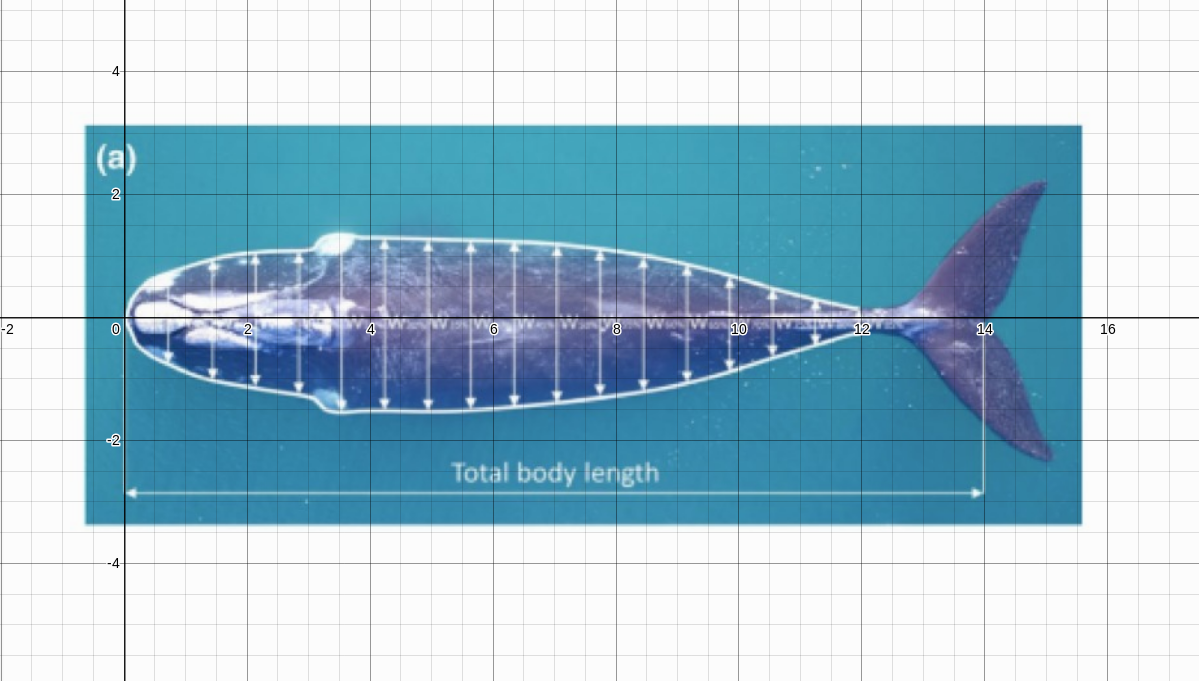
\includegraphics[scale=0.35]{desmos-whale.png}

The \textbf{girth} of the whale at a given point is the circumference of the circular cross-section at this point.

\textbf{2.} From your diagram work out an estimate for the maximum girth of the whale.
\begin{gather*}
  d = 2.9\unit{m} \\
  C = \pi d \\
  C = \pi \times 2.9 \\
  C \approx 9.11\unit{m} \\
\end{gather*}
\ask{$\approx$ necessary?}

\todo{picture showing $d=2.9\unit{m}$}

A formula that can approximate the weight (\textit{M}) of a whale from its size is:
\[
M = 6,144.79 - 1,788B - 914C_{40\%}+500BC_{40\%}
\]

\textbf{3.} Use the formula to estimate the weight of the whale.
\begin{gather*}
  B = 14\unit{m} \\
  C_{40\%} = 9.11\unit{m} \\
  M = 6,144.79 - 1,788B - 914C_{40\%}+500BC_{40\%} \\
  M = 6,144.79 - 1,788 \times 14 - 914 \times 9.11 + 500 \times 14 \times 9.11 \\
  M \approx 36,556 \unit{kg}
\end{gather*}

  Including 5 significant figures is misleading, as it implies a higher precision than the formula can actually give considering the wide variety of whale shapes and densities. I will round my answer to 37,000kg (a precision of two significant figures). \ask{Do I need a justification for this?}

In order to find the average density of a whale an estimate for the volume needs to be calculated.

\textbf{4.}	Find an equation (or equations) that models the upper half of the body of the whale.

I manually placed points every 0.5m along the the upper half of the whale in desmos, then used an online tool to find a polynomial regression. I decided to use 2 equations, one for all points up to 3.5m along the whale, and one for all points after that. Had I only used one equation, I would need a polynomial with a very high degree for an accurate fit because of the bump 3.5m along the whale. I still needed polynomials of degrees 3 and 6, but to model the whale in a single polynomial would have required one of at least degree 13. {\color{red}{Appendix with explanation}}

Here is the equation for $0 \leq x \leq 3.5$:
\begin{equation}
  0.123x^3 - 0.768x^2 + 1.57x + 0.0029
\end{equation}

And here is the equation for $3.5 \leq x \leq 14$:
\begin{equation}
  -0.000044809x^6 + 0.0022276x^5 - 0.0434818x^4 + 0.423465x^3 - 2.17075x^2 + 5.515x - 4
\end{equation}

The high number of decimal places in equation 2 is necessary because of the high exponents involved. With fewer decimal places, the equation strays from the points it should match.

Here is a piecewise function to find the distance of the whale's surface from its line of symmetry, created by combining both equations:
\[
w(x)=
\begin{cases}
  0.123x^3 - 0.768x^2 + 1.57x + 0.0029, & \qquad \text{for} \  0 \leq x \leq 3.5 \\
  -0.000045x^6 + 0.0022x^5 - 0.044x^4 + 0.42x^3 - 2.2x^2 + 5.5x - 4, & \qquad \text{for} \  3.5 \leq x \leq 14
\end{cases}
\]

\vbox{
  Here is an image showing how close $w(x)$ is to the original set of 28 points: \\
  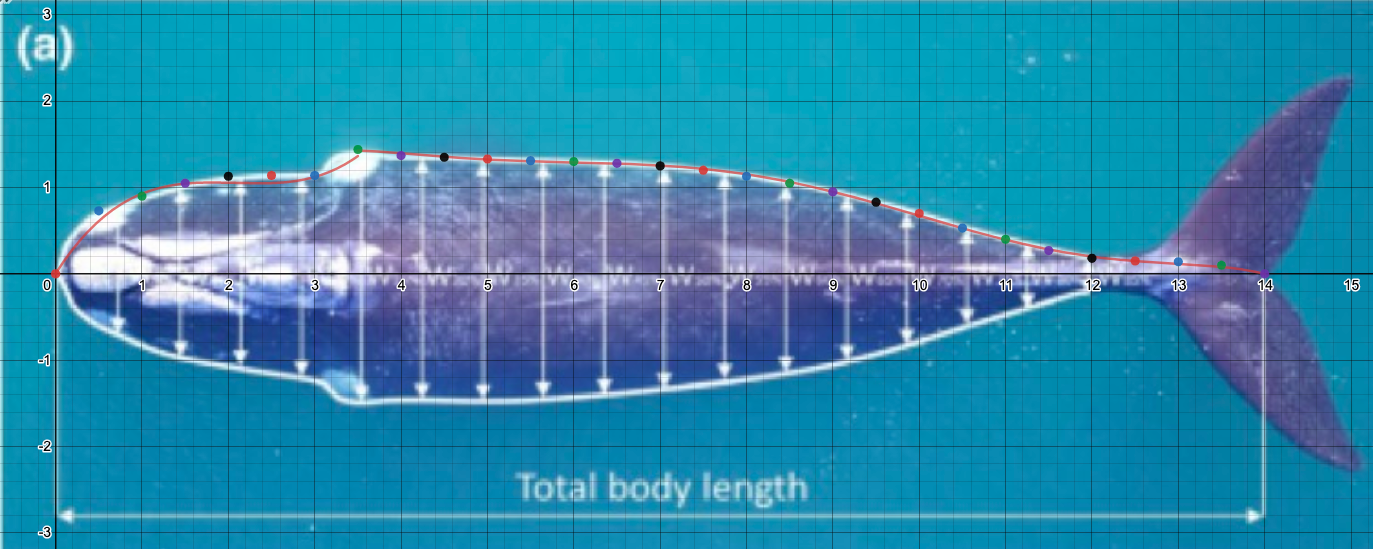
\includegraphics[scale=0.3]{desmos-with-piecewise.png} \\
  \textit{\small$w(x)$ is the red line}
}

\ask{Calculate standard deviation here?}
  
\textbf{5.}	Use a spreadsheet and your model to estimate the distance from the line of symmetry of the whale to the upper edge at intervals of 25 cm.

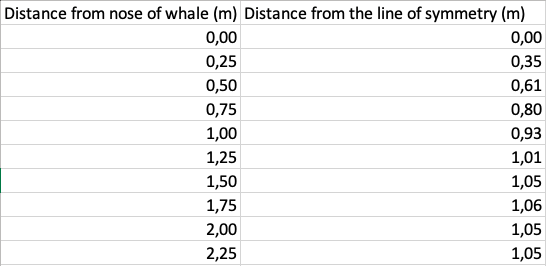
\includegraphics[scale=0.4]{spreadsheet_no_cross.png} \\
\textit{\small First 10 data points, the rest have been cut for brevity}

\textbf{6.}	Find an estimate for the volume of the whale and hence its density. Assume the cross-section of the whale is circular (up to the start of the tail).

One way to approximate the volume of the whale is to compute the cross-sectional area every 0.25m along the length of the whale. Then, we can take the average cross-section and model the whale as a a cylinder with the base of the cylinder being the average previously calculated cross-sectional area.

Assuming all cross-sections of the whale are circular, we can calculate the cross-section by using the formula for the area of a circle, $A=\pi r^2$. We already know $r$, the radius: it is the distance from the line of symmetry, which we calculated in question 5.

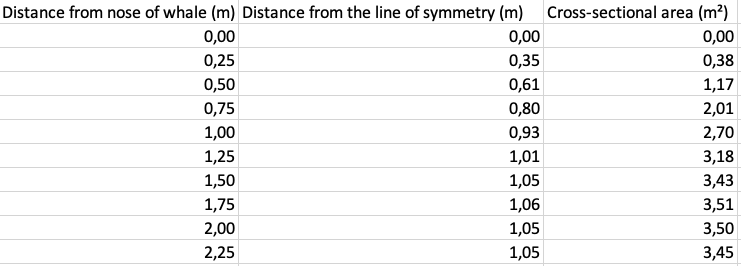
\includegraphics[scale=0.4]{spreadsheet_with_cross.png} \\
\textit{\small The same spreadsheet as in 5., with an additional column for cross-sectional area}

Using excel to calculate the average gives 2.90m$^{2}$. The formula for the area of a cylinder is simply base $\times$ height. The height is the length of the whale's body, 14m, and the base is the 2.90m$^2$ average cross-section of the whale.
\[
V = b \times h = 14 \times 2.9 = 40.6 \unit{m^{3}}
\]
Considering that the whale does not have perfectly circular cross-sections and the volume of the tail was completely ignored, it is misleading to include 3 significant digits. Instead, my answer will be 40m$^3$, with a precision of one significant digit.

The formula for density is $\rho = \frac{m}{V}$ \ask{citation necessary?}. Since we already that know $m$, the mass, is 37,000kg, we can calculate the density of the whale in $\frac{\unit{kg}}{\unit{m^3}}$.
\begin{gather*}
  \rho = \frac{m}{V} \\
  m = 37,000\unit{kg} \\
  V = 40\unit{m^3} \\
  \rho = \frac{37,000}{40} = 925\frac{\unit{kg}}{\unit{m^3}}
\end{gather*}
\ask{when is it correct to include units in calculations?}

\ask{Do I already need to justify the precision of my answer here or can I do it in 7.?}

\todo{try itemize and enumerate}

Does your answer make sense in the context of the problem?

\textbf{7.}	Discuss 

a) The issues particular to the real life problem which may have led to inaccuracies in your answer.  Try to quantify these eg are they likely to lead to your answer being an underestimate or an overestimate?
The biggest potential source of error particular to the real-life problem is that the whale does not have perfeclty circular cross-section. Whales are generally flat \todo{prove it}.

b) Consider the mathematical process used to find the density of the whale.  Which part of the process might lead to inaccuracies in your answer?  Can you quantify these at all?  How might you improve the process to achieve a more accurate answer?

\textbf{8.}	Address one of the sources of error mentioned in question 7 and try to account for it to achieve an improved estimate.


\section{Estimating the surface area of \chry, the Pacific sea nettle}

Use mathematics to find an estimate for the surface area of a whale or a sea creature of your choosing. Your process should include an initial answer and then an identification of an improvement that could be made, which is then carried out. Clearly explain all your steps and discuss, as precisely as you can, any limitations of the process.

I chose to estimate the surface area of \chry. I will only be calculating the area of the dome, not the tentacles, as they have so many subtleties and it is difficult to even define their area.

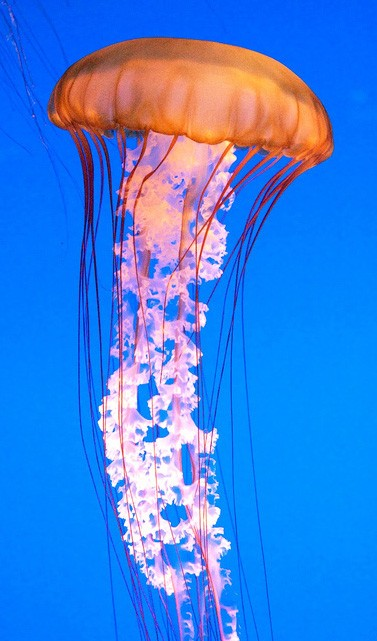
\includegraphics{chrysaora-fuscescens.jpg}

The jellyfish can be modeled as an oblate spheroid, a shape formed by rotating an ellipse around its minor axis. The formula for the surface area of an oblate sphereoid is
\begin{equation*}
  A = 2\pi\left(a^2+\frac{b^2}{\sin(\alpha)}\times\ln\left(\frac{1+\sin(\alpha)}{\cos(\alpha)}\right)\right)
\end{equation*}
where
\begin{equation*}
  \alpha=\arccos\left(\frac{a}{b}\right)
\end{equation*}
$a$ and $b$ are the major and minor axes of the ellipse that forms the spheroid.

\ask{more correct to use square brackets for outer brackets?}
\end{document}
